\chapter{Preliminary implementation} % (fold)
\label{cha:framework}

In this chapter we present our preliminary implementation composited by three
modules: one front-end for the users to iteract with the system, one engine to
choose good job configurations called tuning-by-testing and one back-end to
report the new job configuration.

\section{Overview}

In the Figure~\ref{fig:overview} we show all components together. Fist of all the
user create one file containing initial knobs, this file is submitted to component
front-end which performs lexical, syntatic and semantic analysis on the file, after
it is parsed and sent to engine component. This component, how already explained,
active the BA to choose one good job configuration until reach the criteria. The
result is passed to back-end component that saved in a file.

One interesting feature is the result file can be used as input for the next round
of the self-tuning, just only the user submit it as input. So the framework can work
as incremental software to improve its last result.

\begin{figure}[htbp]
	\centering
	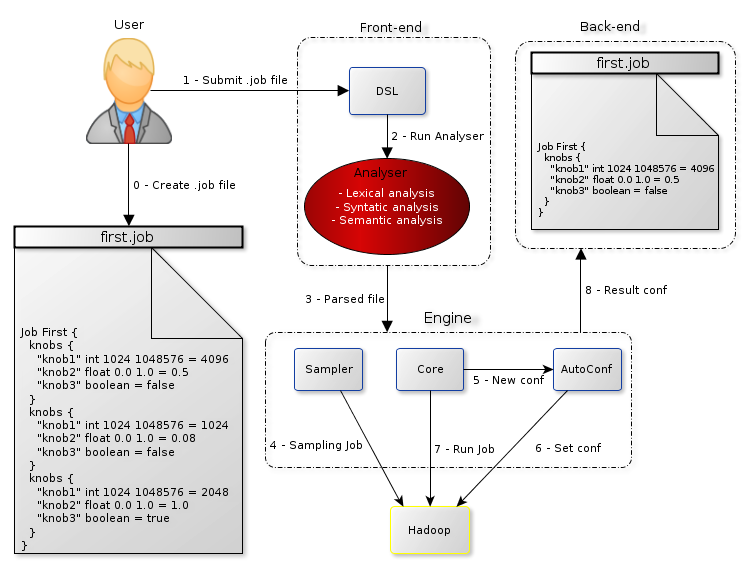
\includegraphics[width=420px,height=330px]{img/overview.png}
	\caption{Implementation overview.}\label{fig:overview}
\end{figure}

\section{Front-end}

The front-end is the {\it DSL} shown in the chapter \ref{cha:dsl}, it consist in
say what is the job name to predict a good configuration and one or several set of
knobs with their initial values, which can be assigned with any values since the
last configuration or rule of thumbs until a random assignment.

One use case of the DSL is shown below, it contains the job name \textbf{WordCount},
its properties and and its set of initial knobs. This set of knobs forms the initial population
for bacteriological algorithm, each set of knob ({\bf knobs}) represents one individual
and one single knob corresponds one gene of individual, any change is done on gene level i.e.
on knob level.

\singlespacing
\begin{listing}[H]
\begin{minted}[mathescape,frame=lines,framesep=2mm,fontfamily=courier,fontsize=\scriptsize]{python}
Job WordCount {
    Properties {
        jarPath /tmp/test/wc/wordcount.jar
        inputHDFSDir /tmp/test/wc/input
        outputHDFSDir /tmp/test/wc/output
        samplePercent 0.2
    }
    knobs {
	    "dfs.block.size" int 1024 1048576 = 4096
	    "io.sort.spill.percent" float 0.0 1.0 = 0.5 
	    "mapred.map.tasks.speculative.execution" boolean = false
    }
    knobs {
	    "dfs.block.size" int 1024 1048576 = 1024
	    "io.sort.spill.percent" float 0.0 1.0 = 0.08
	    "mapred.map.tasks.speculative.execution" boolean = false
    }
    knobs {
	    "dfs.block.size" int 1024 1048576 = 1048576
	    "io.sort.spill.percent" float 0.0 1.0 = 1.0
	    "mapred.map.tasks.speculative.execution" boolean = true
    }
}
\end{minted}
\caption{Usage of DSL Proposal} 
\label{listing:usageDSL}
\end{listing}

As the example shown there are four properties for the job: the jar path, the HDFS
input directory where are stored the input files, the HDFS output directory and the sample
percent. Also there are three initial set of knobs to test, in this example
the first set could be the last job configuration, the second the rule of thumbs
suggested by the comunity and the last one random assignment. However, the users
can interested in testing new knobs that would be easy, just only put a new set
of knobs to test, so this front-end covers enough use cases or combination cases
as much as the users wish.
\newline
\newline
\section{Engine}

The engine is divided in three components: the component to generate
data sample, the component to auto configure hadoop with all configurations generated
by the core component that is responsible for choosing job configurations using BA.

\begin{figure}[htbp]
	\centering
	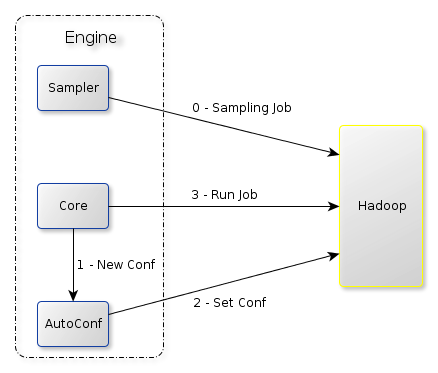
\includegraphics[width=230px,height=200px]{img/engine.png}
	\caption{Engine processing.}\label{fig:engine}
\end{figure}

\subsection{Sampler component}engine

The sampler is responsable to generate data sample, so it sends a command to hadoop
in order to run the sampling job and its output will be used by the core component,
this step is represented by command {\it \bf 0 - Sampling Job}.

\subsection{AutoConf component}

The AutoConf is one component developed by Ramiro, E. %\textcolor{red}{colocar referência do autoconf}
it is responsable for communicate with the hadoop and inject new job configuration,
as seen in the command {\bf 2 - Set Conf}. So independent of configuration files
or configurations assigned for the own job, the hadoop will use job configuration
sent for AutoConf.

\subsection{Core component}

The core component chooses job configurations in order to test its performance
and evaluate the latency time using the bacteriological algorithm, it sends the
command {\bf 1 - New Conf} to component AutoConf after assigned the configuration,
the job is submited to hadoop through the command {\bf Run Job}, then your latency
time is evaluated and the job configuration may added or not to list of good
configurations. The commands sequence {\it 1, 2 and 3} occur until the BA finish,
i.e., until one criteria is reached.

\section{Back-end}

The back-end at the moment is undefined, currently the result is being saved in
one file with the same format of the input file, but with an exception it contains
just the best job configuration found by the BA until the criteria was reached.
